\documentclass[12pt, a4paper, oneside]{ctexart}
\usepackage{amsmath, amsthm, amssymb, bm, color, framed, graphicx, hyperref, mathrsfs, float}

% multi-column
\usepackage{tasks}
% itemize
\NewTasksEnvironment[label=(\arabic*), label-width=3ex]{exercise}

\everymath{\displaystyle}

\title{\textbf{第一次作业}}
\author{U08M11002 Spring 2022}
\date{提交截止日期:北京时间2022年1月24日23:59:59}
\linespread{1}
\definecolor{shadecolor}{RGB}{241, 241, 255}

\newcounter{problemname}
\newenvironment{problem}{\stepcounter{problemname}\par\noindent\textbf{题目\arabic{problemname}. }}{\\\par}
\newenvironment{warning}{\begin{shaded}\par\noindent\textbf{提交作业方式:}}{\end{shaded}\par}

\begin{document}

\maketitle

\begin{warning}
    请于规定截止时间之前将你的作业电子扫描版发送至邮箱 homework@yuxiaoq.in,邮件题目为 「HW1\_张三\_20xxxxxxxx」,其中 20xxxxxxxx 是你的学号。请注意:
   \begin{enumerate}
   	\item 扫描结果应当清晰可见,格式\textbf{必须为单个 pdf 文件};
   	\item 请注意邮件附件大小\textbf{不要超过 10MB};
   	\item 请不要用 QQ 等其他方式发作业给我。
   	\item 超过截止日期提交的作业按照 0 分计算;
   	\item 截止日期前提交的作业若不符合上述要求,或没有被成功接收,视作没有提交作业。
   \end{enumerate}
\end{warning}

\hspace{1em}

\begin{problem}
判断下列各信号是否为周期信号,若为周期信号,求出其周期。
\begin{exercise}(2)
	\task $f(t) = \cos 8t - \sin 12t$
	\task $f(t)  = \cos 2t + 2\sin \pi t$
	\task $f[n] = \cos kn, k \in \mathbb{Z} $
	\task $f[n] = \cos\frac{\pi}{4} n + 2\sin 4\pi n$
\end{exercise}
\quad
\end{problem}

\begin{problem}
试确定下列信号的周期 :
\begin{exercise}(1)
	\task $f(t) = 3\cos(4t+\frac{\pi}{3}) $
	\task $f[n] = 2\cos(\frac{\pi}{4}n) + \sin(\frac{\pi}{8}n)-2\cos(\frac{\pi}{2}n + \frac{\pi}{6}), n \in \mathbb{Z}$
\end{exercise}\quad
\end{problem}

\begin{problem}
判断下列信号是功率信号还是能量信号:
\begin{exercise}(2)
	\task $f(t) = e^{-at} U(t), a > 0$
	\task $f(t) = A \cos (\omega t + \phi)$
	\task $f(t) = tU(t)$
	\task $f[n] = (-0.5)^n U[n]$
	\task $f[n] = U[n]$
\end{exercise}
\quad
\end{problem}

\begin{problem}
求下列积分:
\begin{exercise}(2)
	\task $\int_{-5}^{5} (3t-2)[\delta(t) + \delta(t-2)]dt $
	\task $\int_{-\infty}^{\infty} (2-t)[\delta'(t) + \delta(t)]dt$
	\task $\int_{-5}^{5} (t^2-2t+3) \delta'(t-2)dt$
	\task $\int_{-5}^{1}[\delta(t-2)+\delta(t+4)]\cos\frac{\pi}{2}tdt$
\end{exercise}
\quad
\end{problem}

\begin{problem}
计算下列各题:
\begin{exercise}(2)
	\task $\frac{d^2}{dt^2}[(\cos t + \sin 2t)U(t)]$
	\task $(1-t) \frac{d}{dt}[e^{-t}\delta(t)]$
	\task $\int_{-\infty}^{\infty} \frac{\sin \pi t}{t} \delta(t) dt$
	\task $\int_{-\infty}^{\infty} e^{-2t}[\delta'(t)+\delta(t)]dt$
	\task $\int_{-\infty}^{\infty} [t^2 + \sin \frac{\pi t}{4}] \delta(t+2) dt$
	\task $\int_{-\infty}^{\infty} (t^2+2) \delta(\frac{t}{2})dt$
	\task $\int_{-\infty}^{\infty} (t^3 + 2t^2 - 2t + 1) \delta'(t-1) dt$
	\task $\int_{-\infty}^{t} (1-x)\delta'(x) dx$
\end{exercise}
\quad
\end{problem}

\begin{problem}
画出下列各函数的波形图:
\begin{exercise}(2)
	\task $te^{-t}U(t)$
	\task $e^{-(t-1)}[U(t-1)-U(t-2)]$
	\task $[1+\cos(\pi t)][U(t) - U(t-2)]$
	\task $U(t)-2U(t-1)+U(t-2)$
	\task $\frac{\sin[a(t-t_0)]}{a(t-t_0)}$
	\task $\frac{d}{dt} [e^{-t}(\sin t) U(t)]$
\end{exercise}
\quad
\end{problem}

\newpage
\begin{problem}
已知$f(t)$的波形如下图所示,画出$f(-\frac{1}{2}t - 1)$的波形。
\begin{figure}[H]
	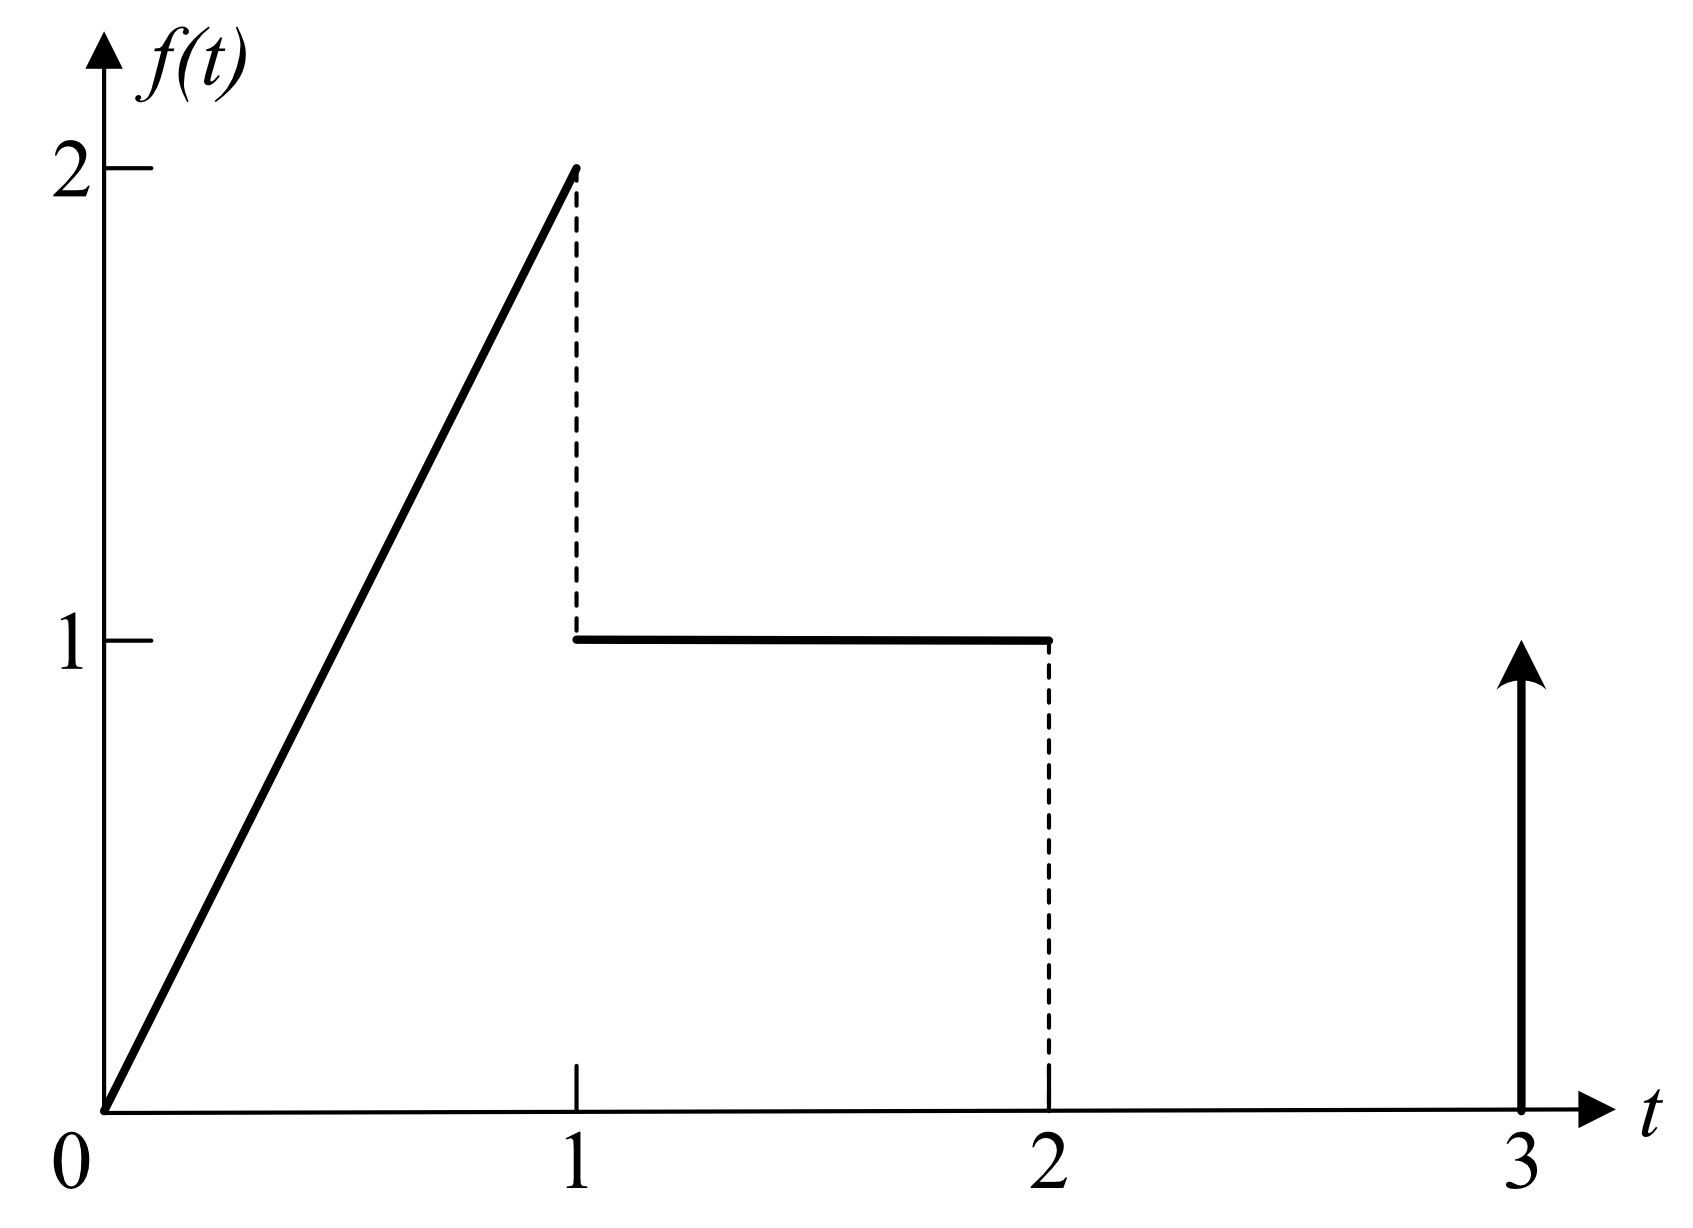
\includegraphics[width=8cm]{assets/hw1img1.png}
	\centering
\end{figure}
\quad
\end{problem}

\begin{problem}
已知$f(t)$的波形如下图所示,画出下列各信号的波形。
\begin{figure}[H]
	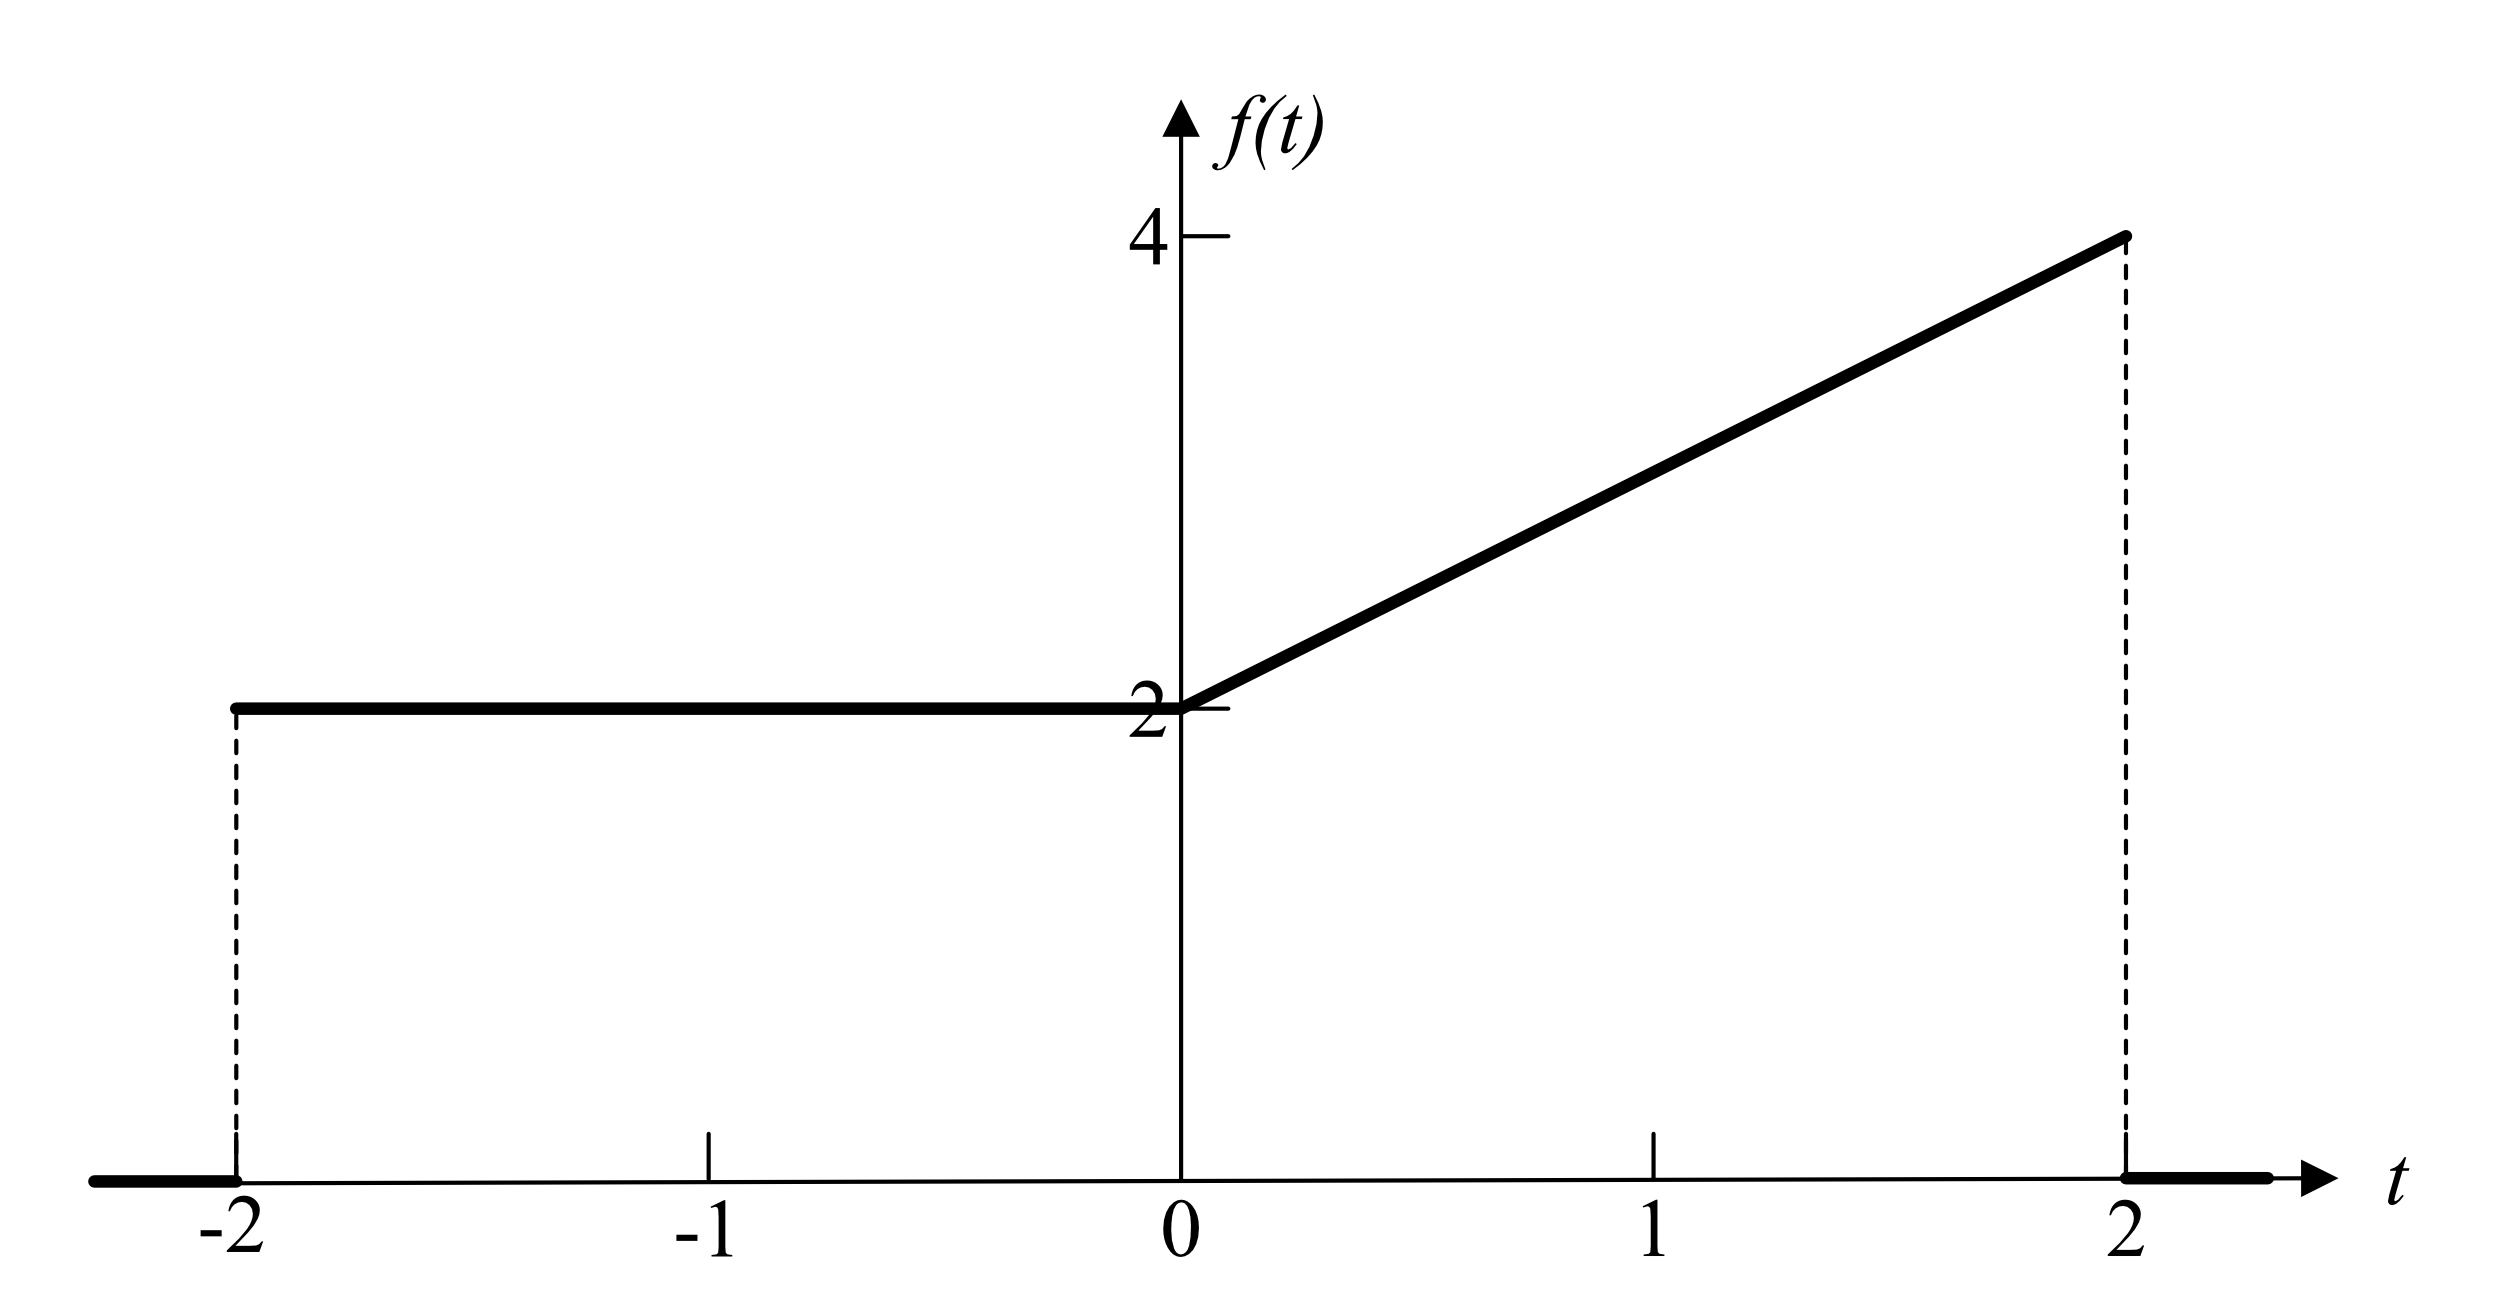
\includegraphics[width=8cm]{assets/hw1img2.png}
	\centering
\end{figure}
\begin{exercise}(2)
	\task $f(t-1)U(t)$
	\task $f(t-1)U(t-1)$
	\task $f(2-t)$
	\task $f(2-t)U(2-t)$
	\task $f(1-2t)$
	\task $f(0.5t-2)$
	\task $\frac{d}{dt} f(t)$
	\task $\int_{-\infty}^{t} f(x) dx$
\end{exercise}
\quad
\end{problem}

\newpage
\begin{problem}
已知信号$f(3-2t)$的波形如下图所示,分别画出$f(t)$和$\frac{d}{dt}f(t)$的波形。
\begin{figure}[h]
	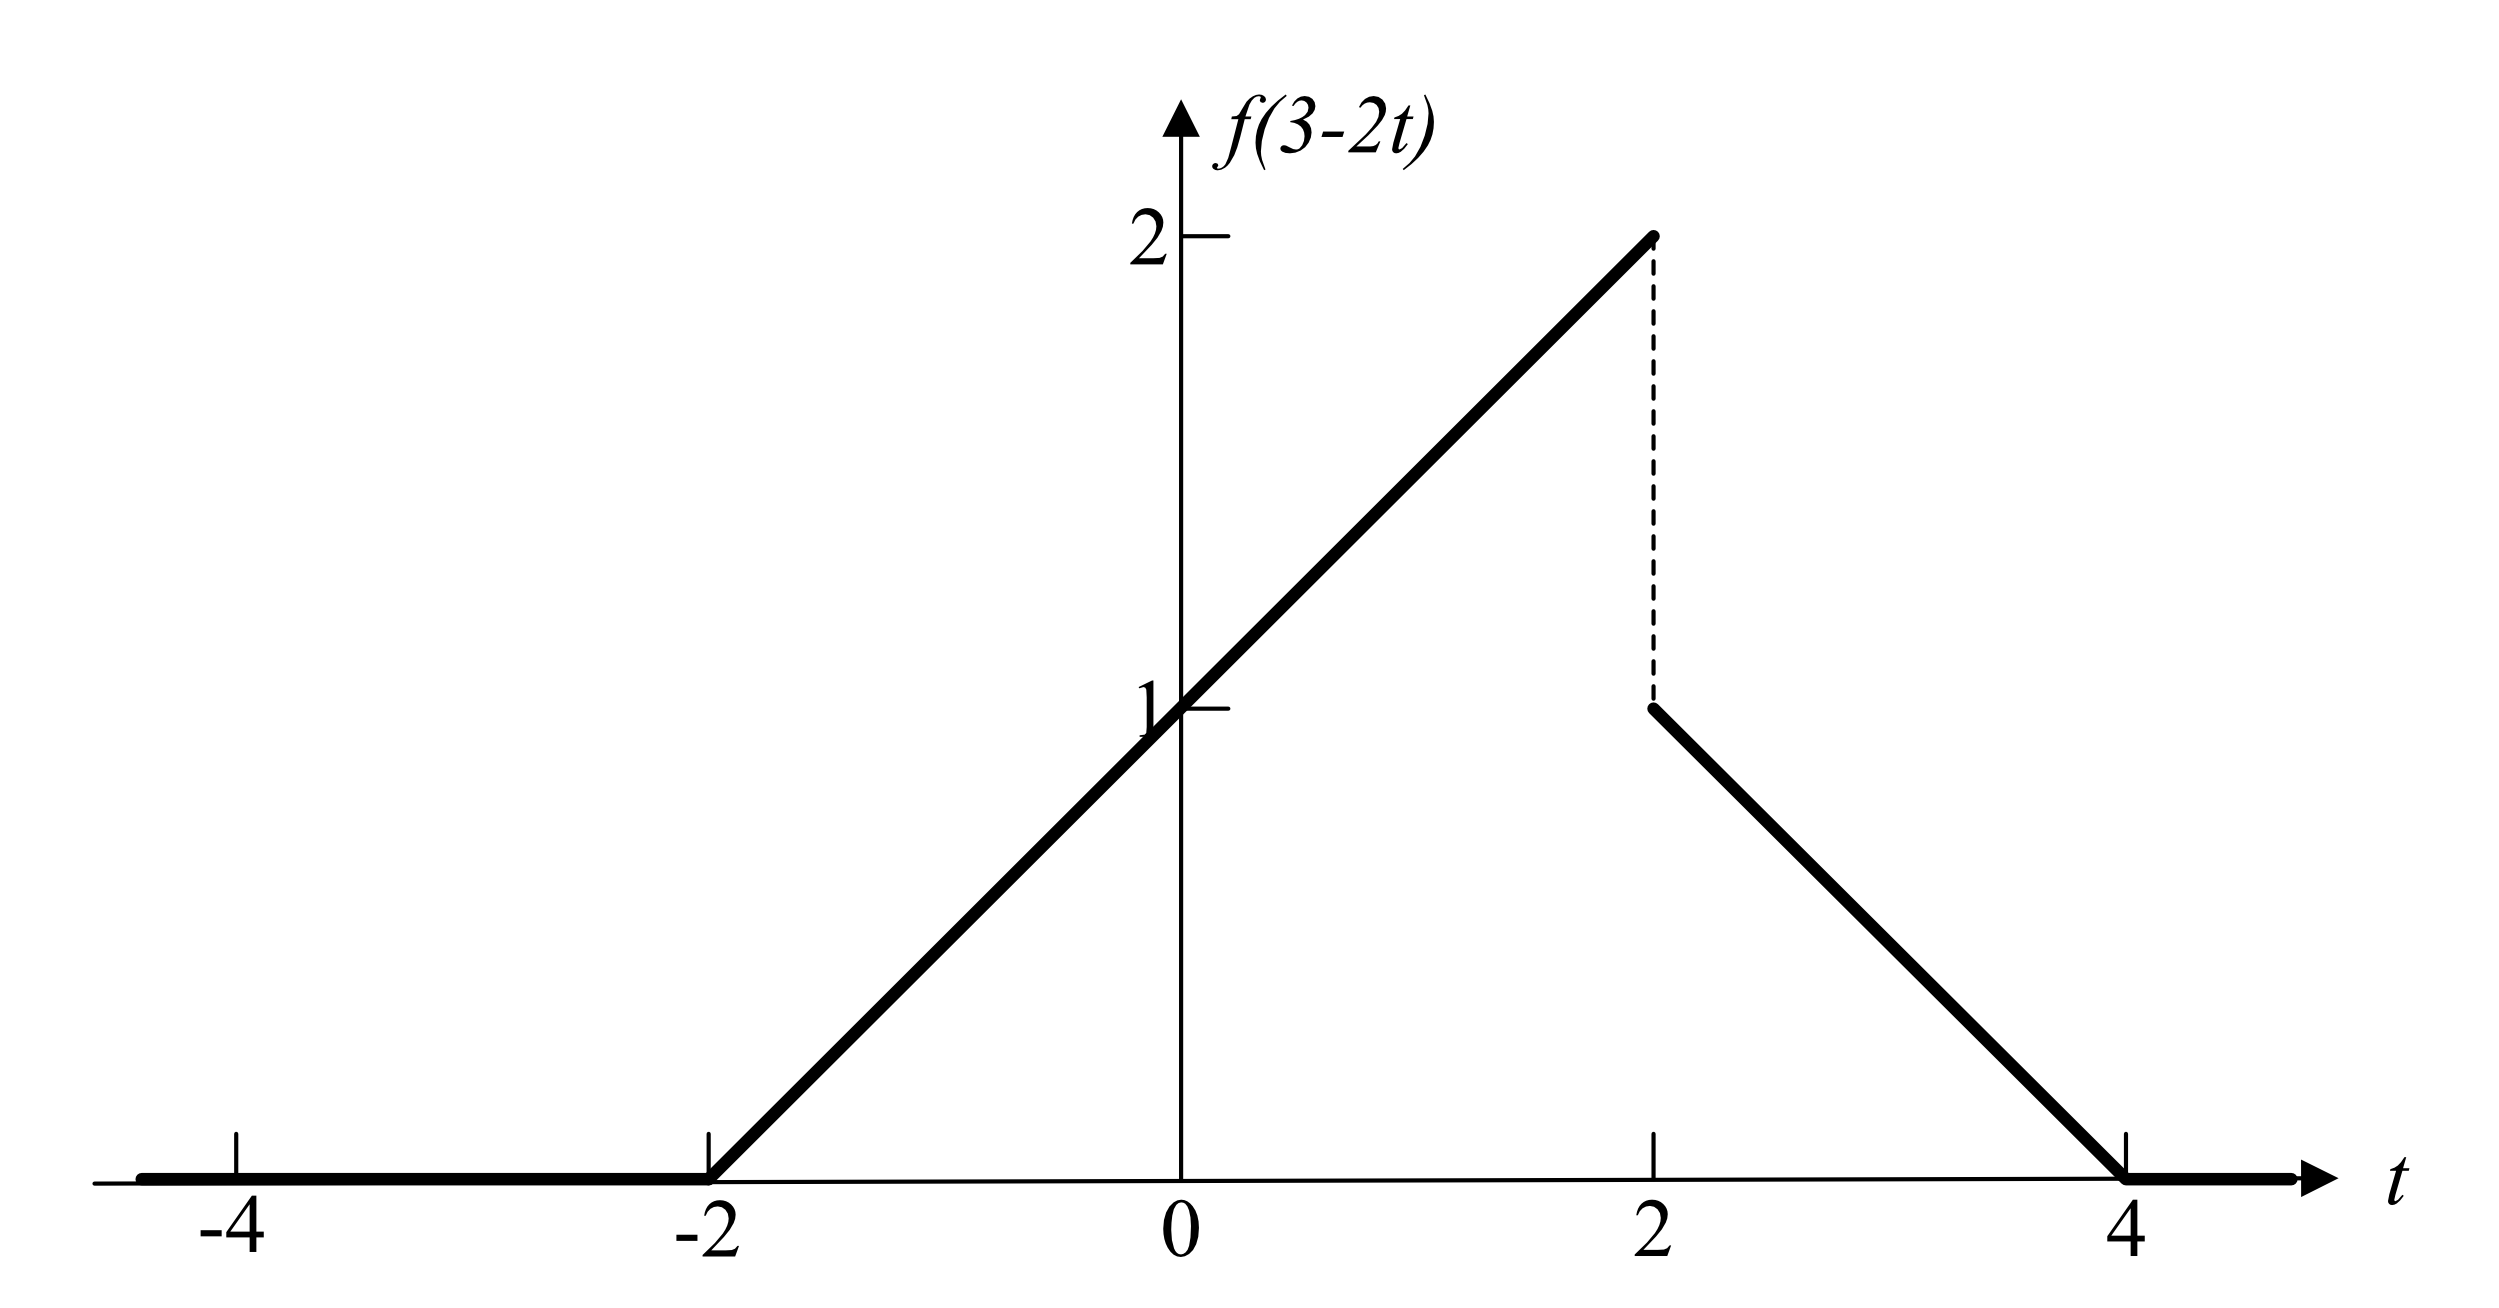
\includegraphics[width=8cm]{assets/hw1img3.png}
	\centering
\end{figure}
\quad
\end{problem}


\begin{problem}
现有如下图所示的电路。请写出:
\begin{figure}[H]
	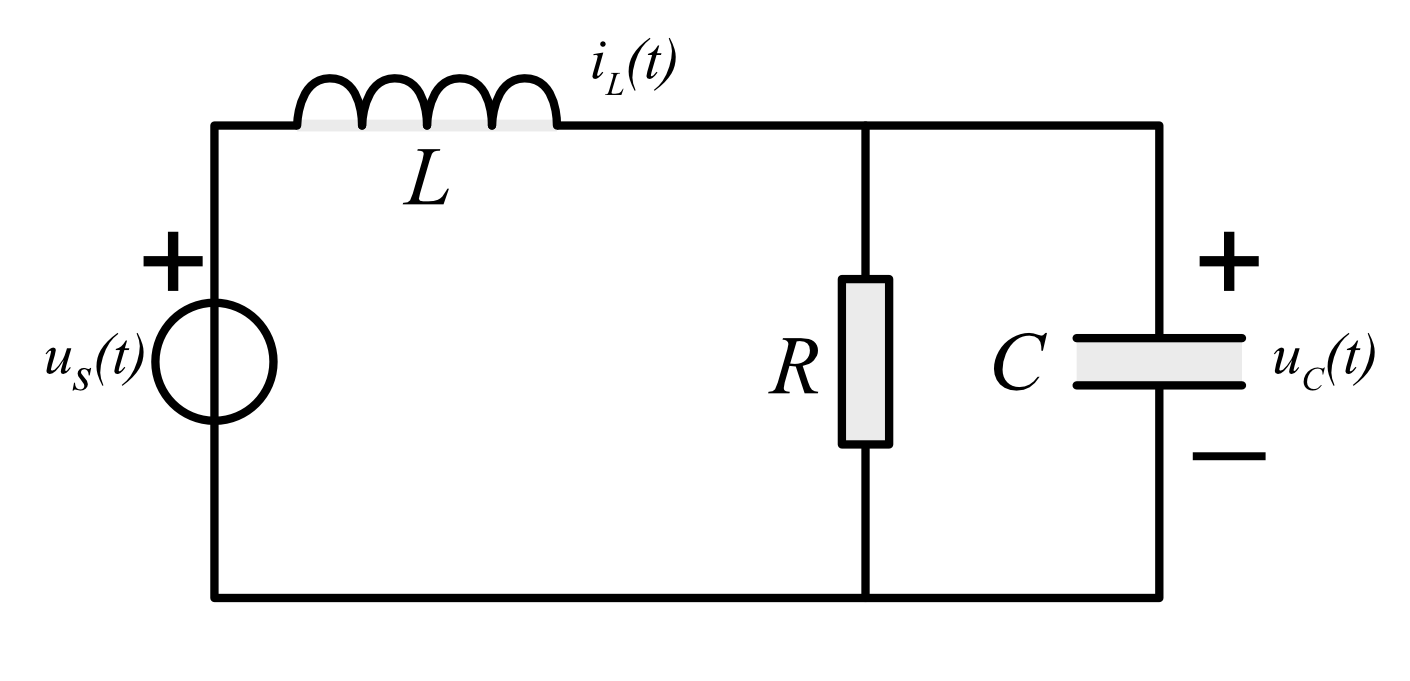
\includegraphics[width=8cm]{assets/hw1img4.png}
	\centering
\end{figure}
\begin{exercise}(1)
	\task 以 $u_{C}(t)$ 为响应的微分方程;
	\task 以 $i_{L}(t)$ 为响应的微分方程。
\end{exercise}

\quad
\end{problem}


































\end{document}